\documentclass{extbook}[14pt]
\usepackage{multicol, enumerate, enumitem, hyperref, color, soul, setspace, parskip, fancyhdr, amssymb, amsthm, amsmath, latexsym, units, mathtools}
\everymath{\displaystyle}
\usepackage[headsep=0.5cm,headheight=0cm, left=1 in,right= 1 in,top= 1 in,bottom= 1 in]{geometry}
\usepackage{dashrule}  % Package to use the command below to create lines between items
\newcommand{\litem}[1]{\item #1

\rule{\textwidth}{0.4pt}}
\pagestyle{fancy}
\lhead{}
\chead{Answer Key for Progress Quiz 4 Version B}
\rhead{}
\lfoot{5346-5907}
\cfoot{}
\rfoot{Summer C 2021}
\begin{document}
\textbf{This key should allow you to understand why you choose the option you did (beyond just getting a question right or wrong). \href{https://xronos.clas.ufl.edu/mac1105spring2020/courseDescriptionAndMisc/Exams/LearningFromResults}{More instructions on how to use this key can be found here}.}

\textbf{If you have a suggestion to make the keys better, \href{https://forms.gle/CZkbZmPbC9XALEE88}{please fill out the short survey here}.}

\textit{Note: This key is auto-generated and may contain issues and/or errors. The keys are reviewed after each exam to ensure grading is done accurately. If there are issues (like duplicate options), they are noted in the offline gradebook. The keys are a work-in-progress to give students as many resources to improve as possible.}

\rule{\textwidth}{0.4pt}

\begin{enumerate}\litem{
Choose the graph of the equation below.
\[ f(x) = \frac{-1}{(x + 1)^2} + 2 \]The solution is the graph below, which is option C.
    \begin{center}
        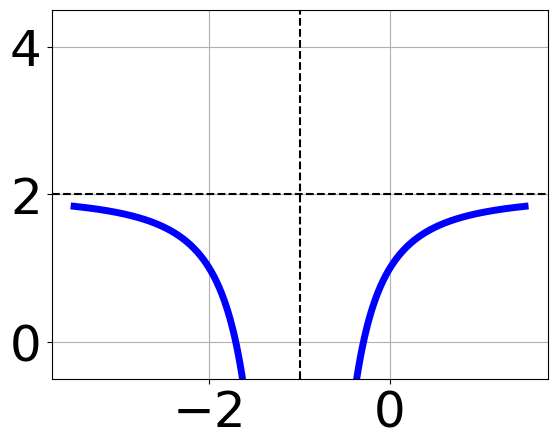
\includegraphics[width=0.3\textwidth]{../Figures/rationalEquationToGraphCB.png}
    \end{center}\begin{enumerate}[label=\Alph*.]
\begin{multicols}{2}
\item 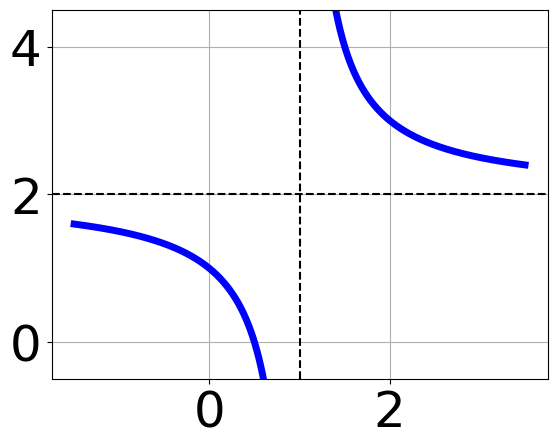
\includegraphics[width = 0.3\textwidth]{../Figures/rationalEquationToGraphAB.png}
\item 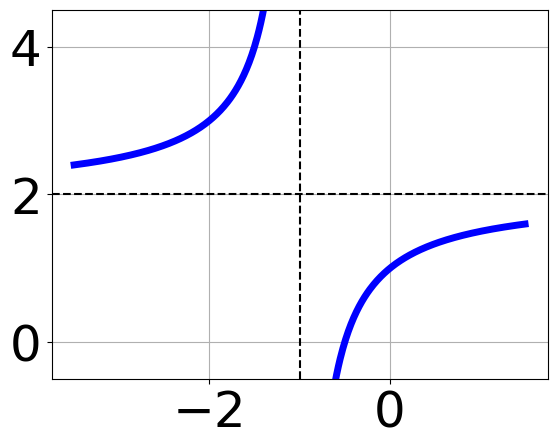
\includegraphics[width = 0.3\textwidth]{../Figures/rationalEquationToGraphBB.png}
\item 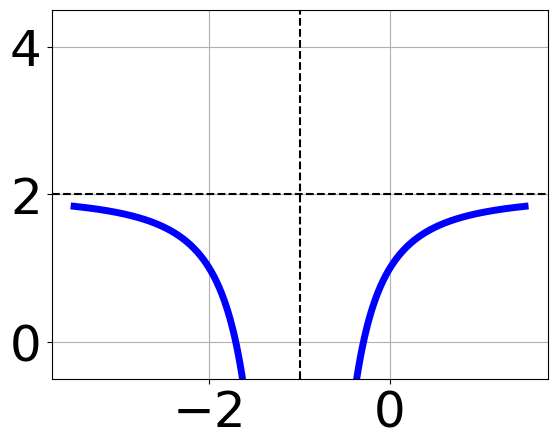
\includegraphics[width = 0.3\textwidth]{../Figures/rationalEquationToGraphCB.png}
\item 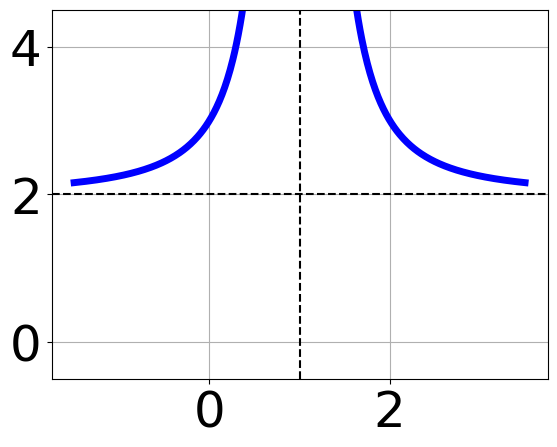
\includegraphics[width = 0.3\textwidth]{../Figures/rationalEquationToGraphDB.png}
\end{multicols}\item None of the above.\end{enumerate}
\textbf{General Comment:} Remember that the general form of a basic rational equation is $ f(x) = \frac{a}{(x-h)^n} + k$, where $a$ is the leading coefficient (and in this case, we assume is either $1$ or $-1$), $n$ is the degree (in this case, either $1$ or $2$), and $(h, k)$ is the intersection of the asymptotes.
}
\litem{
Choose the equation of the function graphed below.

\begin{center}
    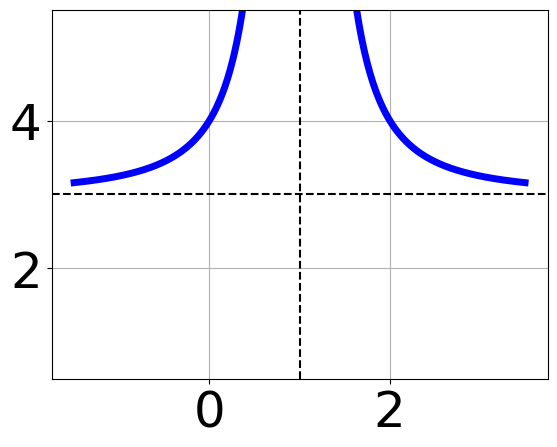
\includegraphics[width=0.5\textwidth]{../Figures/rationalGraphToEquationCopyB.png}
\end{center}


The solution is \( f(x) = \frac{1}{(x - 1)^2} + 3 \), which is option A.\begin{enumerate}[label=\Alph*.]
\item \( f(x) = \frac{1}{(x - 1)^2} + 3 \)

This is the correct option.
\item \( f(x) = \frac{1}{x - 1} + 3 \)

Corresponds to thinking the graph was a shifted version of $\frac{1}{x}$.
\item \( f(x) = \frac{-1}{x + 1} + 3 \)

Corresponds to thinking the graph was a shifted version of $\frac{1}{x}$, using the general form $f(x) = \frac{a}{(x+h)^2}+k$, and the opposite leading coefficient.
\item \( f(x) = \frac{-1}{(x + 1)^2} + 3 \)

Corresponds to using the general form $f(x) = \frac{a}{(x+h)^2}+k$ and the opposite leading coefficient.
\item \( \text{None of the above} \)

This corresponds to believing the vertex of the graph was not correct.
\end{enumerate}

\textbf{General Comment:} Remember that the general form of a basic rational equation is $ f(x) = \frac{a}{(x-h)^n} + k$, where $a$ is the leading coefficient (and in this case, we assume is either $1$ or $-1$), $n$ is the degree (in this case, either $1$ or $2$), and $(h, k)$ is the intersection of the asymptotes.
}
\litem{
Choose the equation of the function graphed below.

\begin{center}
    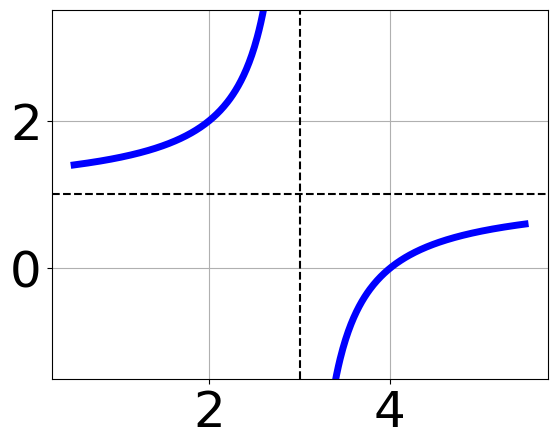
\includegraphics[width=0.5\textwidth]{../Figures/rationalGraphToEquationB.png}
\end{center}


The solution is \( f(x) = \frac{-1}{x - 3} + 1 \), which is option A.\begin{enumerate}[label=\Alph*.]
\item \( f(x) = \frac{-1}{x - 3} + 1 \)

This is the correct option.
\item \( f(x) = \frac{-1}{(x - 3)^2} + 1 \)

Corresponds to thinking the graph was a shifted version of $\frac{1}{x^2}$.
\item \( f(x) = \frac{1}{x + 3} + 1 \)

Corresponds to using the general form $f(x) = \frac{a}{x+h}+k$ and the opposite leading coefficient.
\item \( f(x) = \frac{1}{(x + 3)^2} + 1 \)

Corresponds to thinking the graph was a shifted version of $\frac{1}{x^2}$, using the general form $f(x) = \frac{a}{x+h}+k$, and the opposite leading coefficient.
\item \( \text{None of the above} \)

This corresponds to believing the vertex of the graph was not correct.
\end{enumerate}

\textbf{General Comment:} Remember that the general form of a basic rational equation is $ f(x) = \frac{a}{(x-h)^n} + k$, where $a$ is the leading coefficient (and in this case, we assume is either $1$ or $-1$), $n$ is the degree (in this case, either $1$ or $2$), and $(h, k)$ is the intersection of the asymptotes.
}
\litem{
Solve the rational equation below. Then, choose the interval(s) that the solution(s) belongs to.
\[ \frac{-56}{-35x -14} + 1 = \frac{-56}{-35x -14} \]The solution is \( \text{all solutions are invalid or lead to complex values in the equation.} \), which is option C.\begin{enumerate}[label=\Alph*.]
\item \( x \in [-0.4,0.6] \)

$x = -0.400$, which corresponds to not checking if this value leads to dividing by 0 in the original equation and thus is not a valid solution.
\item \( x_1 \in [-1.3, -0.3] \text{ and } x_2 \in [0.2,1.2] \)

$x = -0.400 \text{ and } x = 0.400$, which corresponds to getting the correct solution and believing there should be a second solution to the equation.
\item \( \text{All solutions lead to invalid or complex values in the equation.} \)

*$x = -0.400$ leads to dividing by 0 in the original equation and thus is not a valid solution, which is the correct option.
\item \( x \in [0.3,1.6] \)

$x = 0.400$, which corresponds to not distributing the factor $-35x -14$ correctly when trying to eliminate the fraction.
\item \( x_1 \in [-1.3, -0.3] \text{ and } x_2 \in [-1.5,-0.1] \)

$x = -0.400 \text{ and } x = -0.400$, which corresponds to getting the correct solution and believing there should be a second solution to the equation.
\end{enumerate}

\textbf{General Comment:} Distractors are different based on the number of solutions. Remember that after solving, we need to make sure our solution does not make the original equation divide by zero!
}
\litem{
Solve the rational equation below. Then, choose the interval(s) that the solution(s) belongs to.
\[ \frac{-7x}{2x -3} + \frac{-5x^{2}}{12x^{2} -24 x + 9} = \frac{-4}{6x -3} \]The solution is \( \text{All solutions are invalid or lead to complex values in the equation.} \), which is option C.\begin{enumerate}[label=\Alph*.]
\item \( x \in [-0.77,0.63] \)

$x = 0.500$, which corresponds to solving $6x -3 = 0$ and treating it as a solution to the equation.
\item \( x_1 \in [0.55, 1.03] \text{ and } x_2 \in [-0.16,0.48] \)

$x = 0.805 \text{ and } x = -0.021$, which corresponds to making the discriminant from the Quadratic Formula positive to avoid complex solutions.
\item \( \text{All solutions lead to invalid or complex values in the equation.} \)

* The equation leads to solving $-37x^{2} +29 x -12=0$, which leads to complex solutions. This is the correct option.
\item \( x_1 \in [0.82, 2.19] \text{ and } x_2 \in [0.46,0.85] \)

$x = 1.500 \text{ and } x = 0.500$, which corresponds to solving $2x -3 = 0$ and $6x -3 = 0$ and treating them as solutions to the equation.
\item \( x \in [0.82,2.19] \)

$x = 1.500$, which corresponds to solving $2x -3 = 0$ and treating it as a solution to the equation.
\end{enumerate}

\textbf{General Comment:} Distractors are different based on the number of solutions. Remember that after solving, we need to make sure our solution does not make the original equation divide by zero!
}
\litem{
Determine the domain of the function below.
\[ f(x) = \frac{5}{20x^{2} -5 x -25} \]The solution is \( \text{All Real numbers except } x = -1.000 \text{ and } x = 1.250. \), which is option E.\begin{enumerate}[label=\Alph*.]
\item \( \text{All Real numbers except } x = a, \text{ where } a \in [-25, -23] \)

All Real numbers except $x = -25.000$, which corresponds to removing a distractor value from the denominator.
\item \( \text{All Real numbers except } x = a, \text{ where } a \in [-1, 1] \)

All Real numbers except $x = -1.000$, which corresponds to removing only 1 value from the denominator.
\item \( \text{All Real numbers.} \)

This corresponds to thinking the denominator has complex roots or that rational functions have a domain of all Real numbers.
\item \( \text{All Real numbers except } x = a \text{ and } x = b, \text{ where } a \in [-25, -23] \text{ and } b \in [19, 23] \)

All Real numbers except $x = -25.000$ and $x = 20.000$, which corresponds to not factoring the denominator correctly.
\item \( \text{All Real numbers except } x = a \text{ and } x = b, \text{ where } a \in [-1, 1] \text{ and } b \in [1.25, 2.25] \)

All Real numbers except $x = -1.000$ and $x = 1.250$, which is the correct option.
\end{enumerate}

\textbf{General Comment:} Recall that dividing by zero is not a real number. Therefore the domain is all real numbers \textbf{except} those that make the denominator 0.
}
\litem{
Solve the rational equation below. Then, choose the interval(s) that the solution(s) belongs to.
\[ \frac{5}{-4x -2} + -7 = \frac{3}{36x + 18} \]The solution is \( x = -0.690 \), which is option D.\begin{enumerate}[label=\Alph*.]
\item \( x \in [0.1,1.4] \)

$x = 0.310$, which corresponds to not distributing the factor $-4x -2$ correctly when trying to eliminate the fraction.
\item \( x_1 \in [-0.8, -0.2] \text{ and } x_2 \in [-0.4,2.1] \)

$x = -0.690 \text{ and } x = 0.310$, which corresponds to getting the correct solution and believing there should be a second solution to the equation.
\item \( x_1 \in [-0.8, -0.2] \text{ and } x_2 \in [-0.8,0.2] \)

$x = -0.690 \text{ and } x = -0.571$, which corresponds to getting the correct solution and believing there should be a second solution to the equation.
\item \( x \in [-0.69,0.31] \)

* $x = -0.690$, which is the correct option.
\item \( \text{All solutions lead to invalid or complex values in the equation.} \)

This corresponds to thinking $x = -0.690$ leads to dividing by zero in the original equation, which it does not.
\end{enumerate}

\textbf{General Comment:} Distractors are different based on the number of solutions. Remember that after solving, we need to make sure our solution does not make the original equation divide by zero!
}
\litem{
Solve the rational equation below. Then, choose the interval(s) that the solution(s) belongs to.
\[ \frac{4x}{2x + 2} + \frac{-7x^{2}}{-12x^{2} -6 x + 6} = \frac{-4}{-6x + 3} \]The solution is \( \text{There are two solutions: } x = -0.279 \text{ and } x = 0.924 \), which is option E.\begin{enumerate}[label=\Alph*.]
\item \( \text{All solutions lead to invalid or complex values in the equation.} \)


\item \( x \in [0.69,0.98] \)


\item \( x_1 \in [-0.64, 0.28] \text{ and } x_2 \in [-1.7,-0.8] \)


\item \( x \in [-0.08,0.57] \)


\item \( x_1 \in [-0.64, 0.28] \text{ and } x_2 \in [-0.8,1.7] \)

* $x = -0.279 \text{ and } x = 0.924$, which is the correct option.
\end{enumerate}

\textbf{General Comment:} Distractors are different based on the number of solutions. Remember that after solving, we need to make sure our solution does not make the original equation divide by zero!
}
\litem{
Choose the graph of the equation below.
\[ f(x) = \frac{1}{x - 3} - 1 \]The solution is the graph below, which is option D.
    \begin{center}
        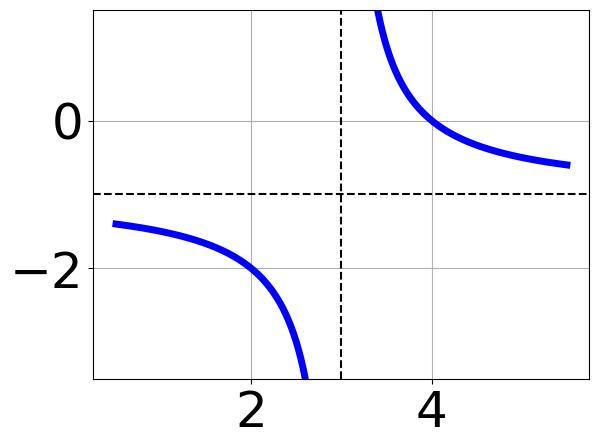
\includegraphics[width=0.3\textwidth]{../Figures/rationalEquationToGraphCopyDB.png}
    \end{center}\begin{enumerate}[label=\Alph*.]
\begin{multicols}{2}
\item 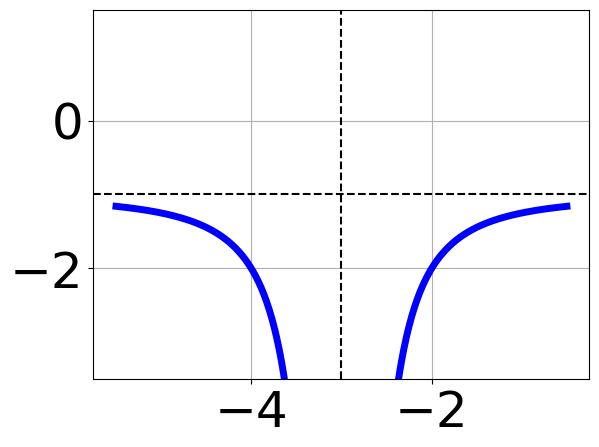
\includegraphics[width = 0.3\textwidth]{../Figures/rationalEquationToGraphCopyAB.png}
\item 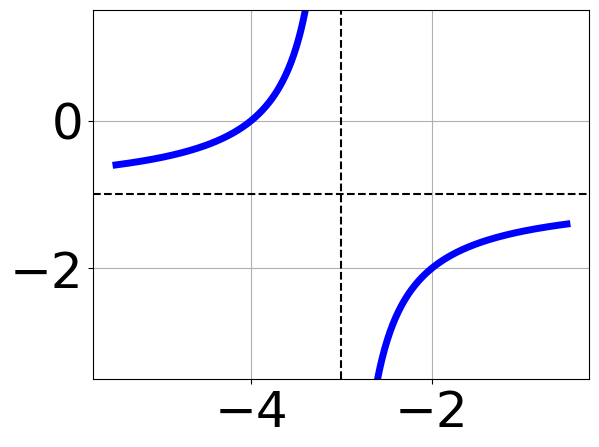
\includegraphics[width = 0.3\textwidth]{../Figures/rationalEquationToGraphCopyBB.png}
\item 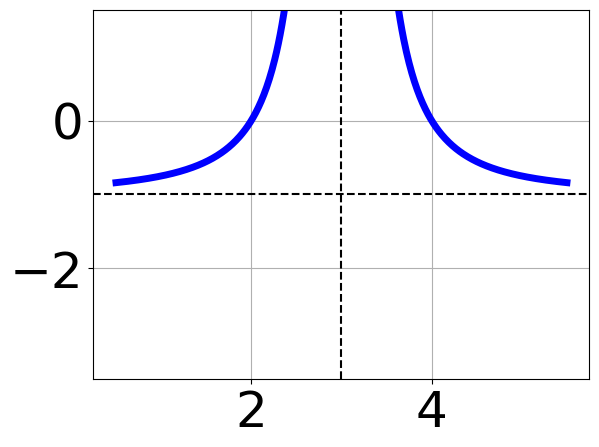
\includegraphics[width = 0.3\textwidth]{../Figures/rationalEquationToGraphCopyCB.png}
\item 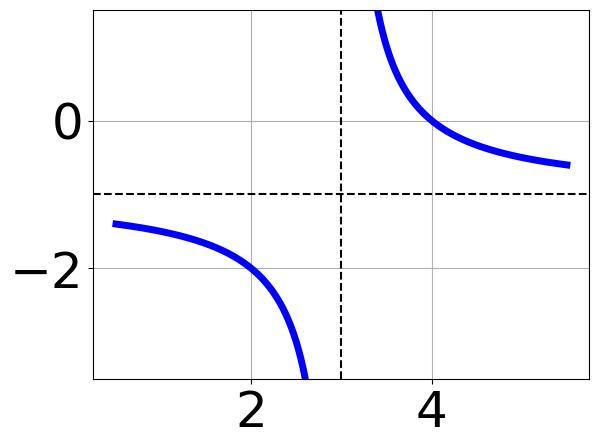
\includegraphics[width = 0.3\textwidth]{../Figures/rationalEquationToGraphCopyDB.png}
\end{multicols}\item None of the above.\end{enumerate}
\textbf{General Comment:} Remember that the general form of a basic rational equation is $ f(x) = \frac{a}{(x-h)^n} + k$, where $a$ is the leading coefficient (and in this case, we assume is either $1$ or $-1$), $n$ is the degree (in this case, either $1$ or $2$), and $(h, k)$ is the intersection of the asymptotes.
}
\litem{
Determine the domain of the function below.
\[ f(x) = \frac{5}{20x^{2} +9 x -20} \]The solution is \( \text{All Real numbers except } x = -1.250 \text{ and } x = 0.800. \), which is option B.\begin{enumerate}[label=\Alph*.]
\item \( \text{All Real numbers except } x = a, \text{ where } a \in [-2.25, -0.25] \)

All Real numbers except $x = -1.250$, which corresponds to removing only 1 value from the denominator.
\item \( \text{All Real numbers except } x = a \text{ and } x = b, \text{ where } a \in [-2.25, -0.25] \text{ and } b \in [0.8, 3.8] \)

All Real numbers except $x = -1.250$ and $x = 0.800$, which is the correct option.
\item \( \text{All Real numbers.} \)

This corresponds to thinking the denominator has complex roots or that rational functions have a domain of all Real numbers.
\item \( \text{All Real numbers except } x = a, \text{ where } a \in [-20, -19] \)

All Real numbers except $x = -20.000$, which corresponds to removing a distractor value from the denominator.
\item \( \text{All Real numbers except } x = a \text{ and } x = b, \text{ where } a \in [-20, -19] \text{ and } b \in [17, 24] \)

All Real numbers except $x = -20.000$ and $x = 20.000$, which corresponds to not factoring the denominator correctly.
\end{enumerate}

\textbf{General Comment:} Recall that dividing by zero is not a real number. Therefore the domain is all real numbers \textbf{except} those that make the denominator 0.
}
\end{enumerate}

\end{document}